\paragraph*{Primo Impatto}
Disastrosa la situazione al primo impatto col sito. Come visibile in \autoref{fig:HomeFirstCut}, il sito risulta "tagliato" dalla schermata. Ciò comporta la necessità per l'utente di scrollare (\fullref{par:Scrolling}). Il tutto è aggravato dal fatto che ad occupare la maggior parte dello spazio sono immagini totalmente inutili. La situazione non migliora troppo andando a diminuire la larghezza dello schermo, che comporta una riduzione nell'altezza delle immagini.
Il layout tagliato comporta anche una difficoltà per l'utente nel crearsi una mappa mentale completa. I pochi rifermenti che trova sono:
\begin{itemize}
	\item Il logo del sito.
	\item I link del menu (abbastanza criptici, ad eccezione di \textit{"sistemi e prodotti"}).
	\item La frase emozionale che passa con l'immagine di turno.
\end{itemize}
%


\begin{figure}
	\centering
	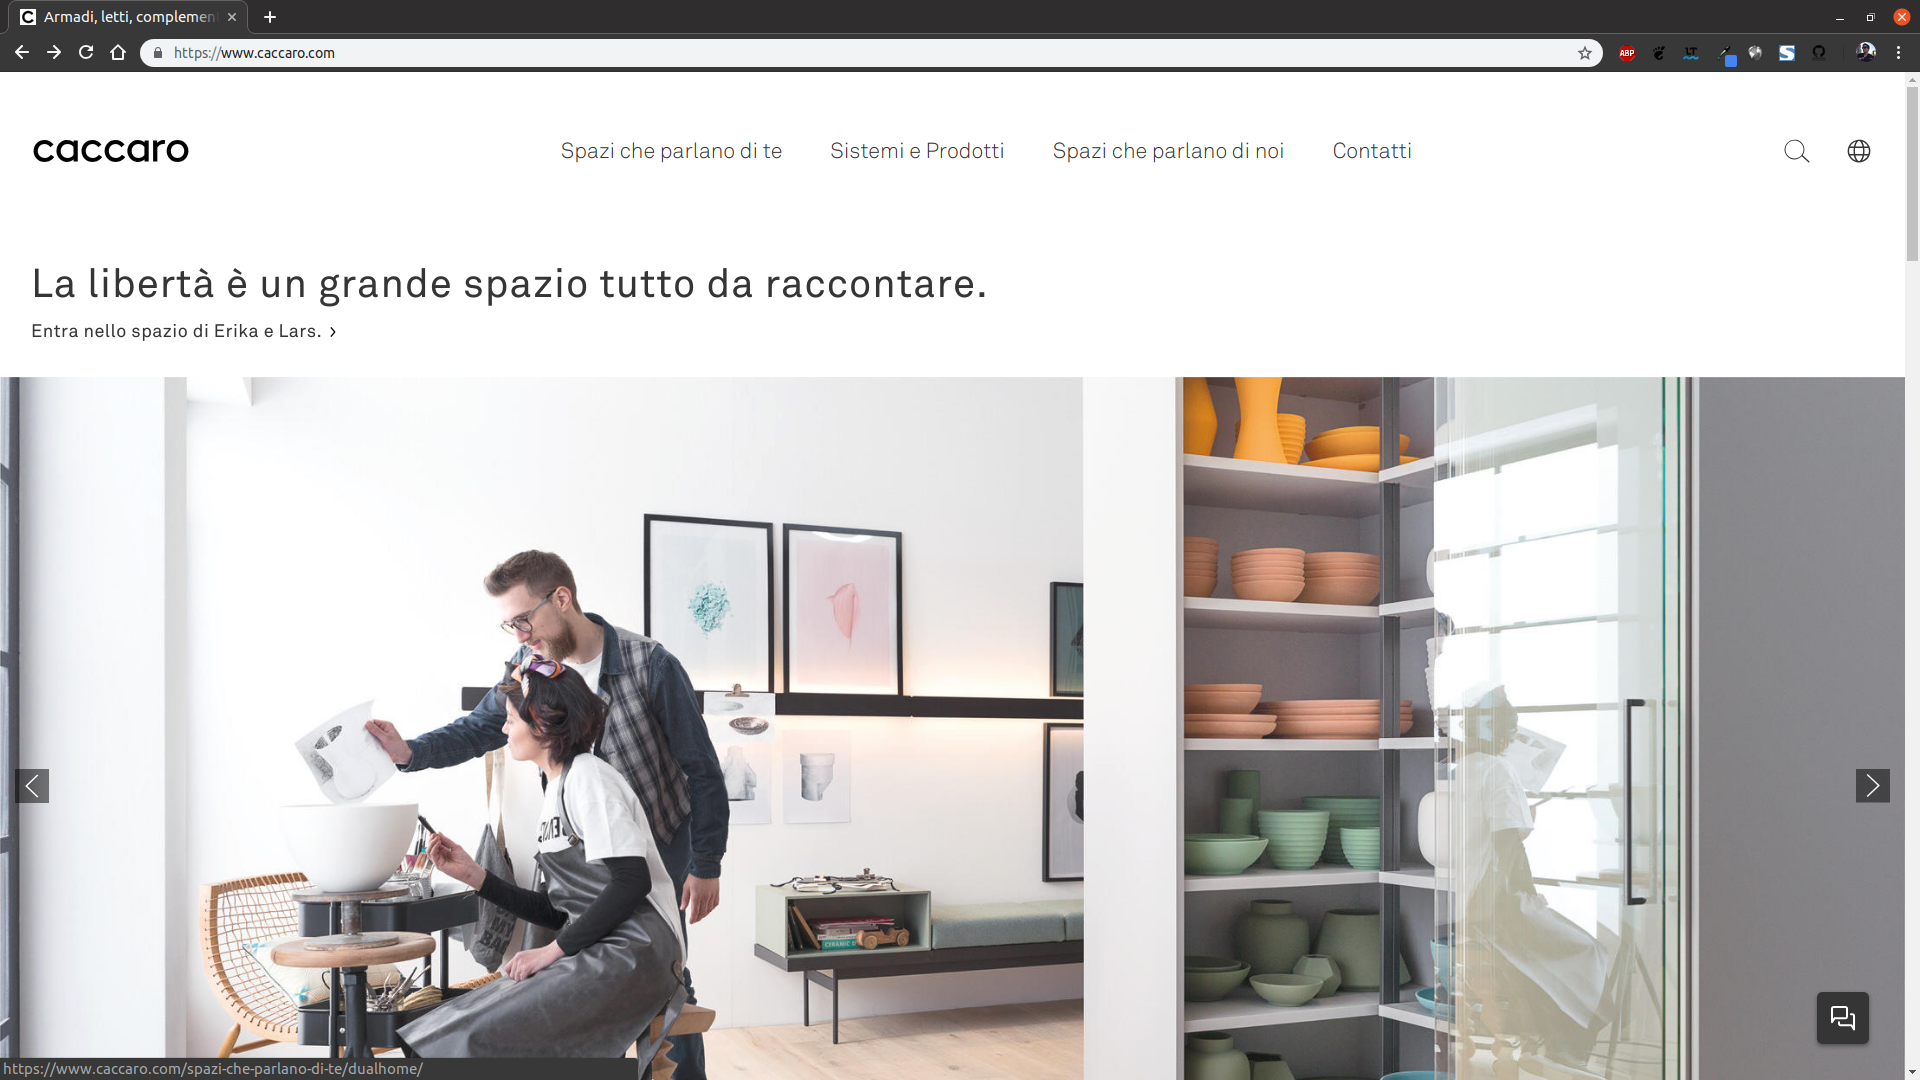
\includegraphics[width=\textwidth]{sez/HomePage/img/HomeFirstCut.png}
	\caption[https://www.caccaro.com/]{First cut della home: l'immagine spreca tutto lo spazio a disposizione}
	\label{fig:HomeFirstCut}
\end{figure}

\paragraph*{Contenuto e Scrolling}
\label{par:Scrolling}
Per consultare l'intera homepage sono necessarie quattro schermate di scrolling, decisamente troppo considerando che il 77\% degli utenti non scrolla nella schermata principale. Sostanzialmente, i veri contenuti della pagina non vengono mai visti, rendendo la homepage veramente poco efficace.\newline
Analizziamo dunque le cause di questo scrolling eccessivo:
\begin{itemize}
	\item \textbf{Troppo testo:} In una homepage è consigliato non andare oltre le 93 parole a schermo, ovvero tutte quelle che un utente riesce a leggere durante sua prima visita (circa 31 secondi). Senza contare gli elementi di navigazione, nella homepage di Caccaro ne sono presenti molto più del doppio. \`E sicuramente necessario uno sfoltimento dei contenuti.
	\item \textbf{Layout troppo diluito:} Un layout diluito può aiutare l'utente a crearsi una mappa mentale. In questo caso però lo è veramente troppo: le immagini occupano troppo spazio e di conseguenza ci sono enormi spaziature fra i paragrafi (sono questi gli spazi che parlano di me? \autoref{fig:Spazi}). Il layout sembra più quello di un catalogo che quello di un sito.
\end{itemize}

\begin{figure}[H]
	\centering
	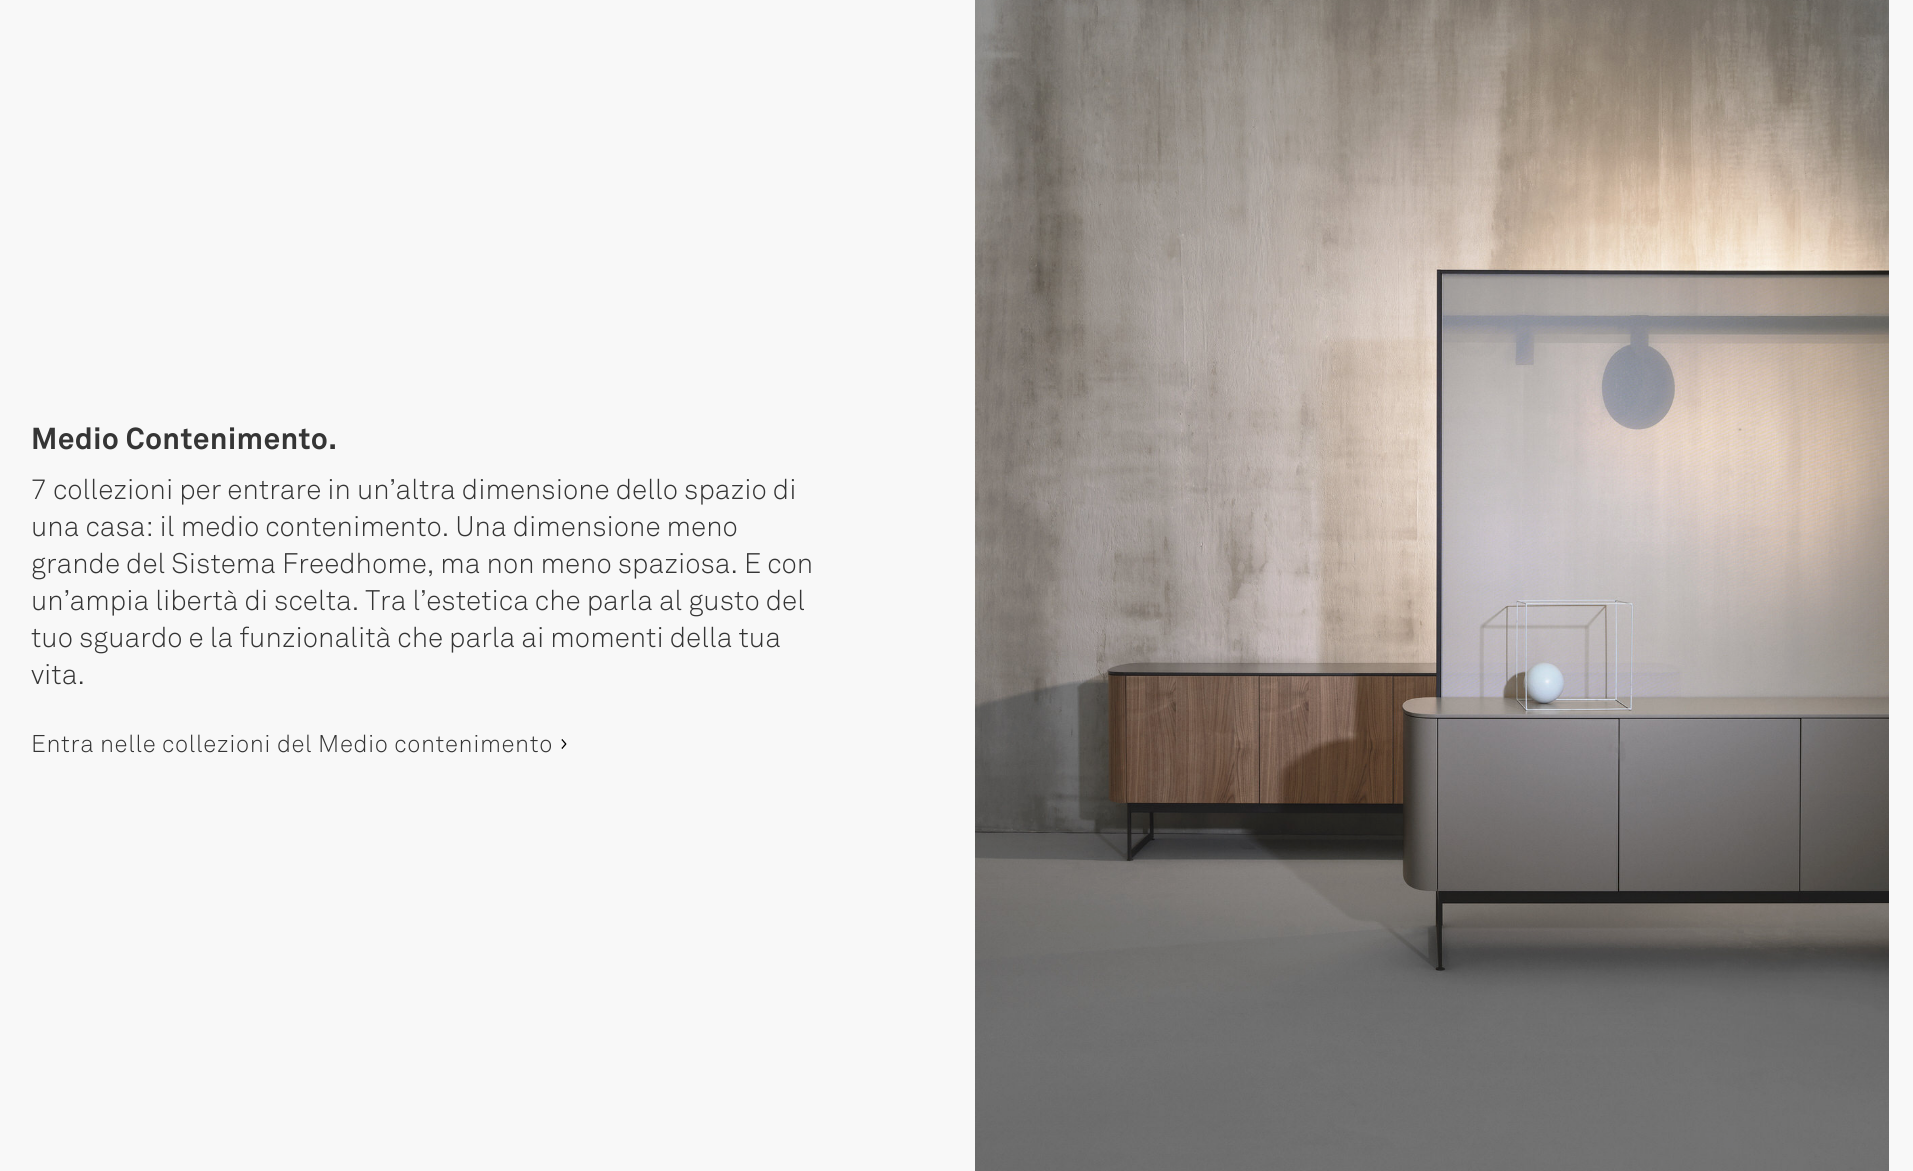
\includegraphics[width=\textwidth]{sez/HomePage/img/Spazi.png}
	\caption[https://www.caccaro.com/]{Sezione della home: spazi vuoti e immagini di dimensioni esagerate (l'immagine è più alta di una schermata)}
	\label{fig:Spazi}
\end{figure}

%Perche' scrolling: troppo testo, immagini gigantesche, roba emozionale inutile, layout alla cazzo di cane

\paragraph*{Immagini}
Bisogna partire da questo presupposto: sul web le immagini sono meno importanti del testo. L'attenzione dell'utente si sofferma molto di più sulle informazioni contenute nei paragrafi.
Risulta quindi particolarmente inefficace la scelta di tappezzare la home con figure di dimensioni esagerate.\\
Le immagini sono comunque necessarie per mostrare subito all'utente i prodotti: bene quindi quelle che sono accompagnate dai paragrafi "Sistema FreedHome", "Letti" e "Medio contenimento", che mostrano chiaramente gli articoli. Peggio invece le immagini nel first cut (le più importanti!), dalle quali un utente qualsiasi non può capire cosa Caccaro abbia da offrire. Criptica, per non dire altro, l'immagine in \autoref{fig:Blocchetti}.\\
Bene il fatto che tutte le immagini siano cliccabili, in quanto l'utente tende spesso a cliccare sulle immagini e si aspetta di venire portato a una pagina interna del sito.

\begin{figure}[H]
	\centering
	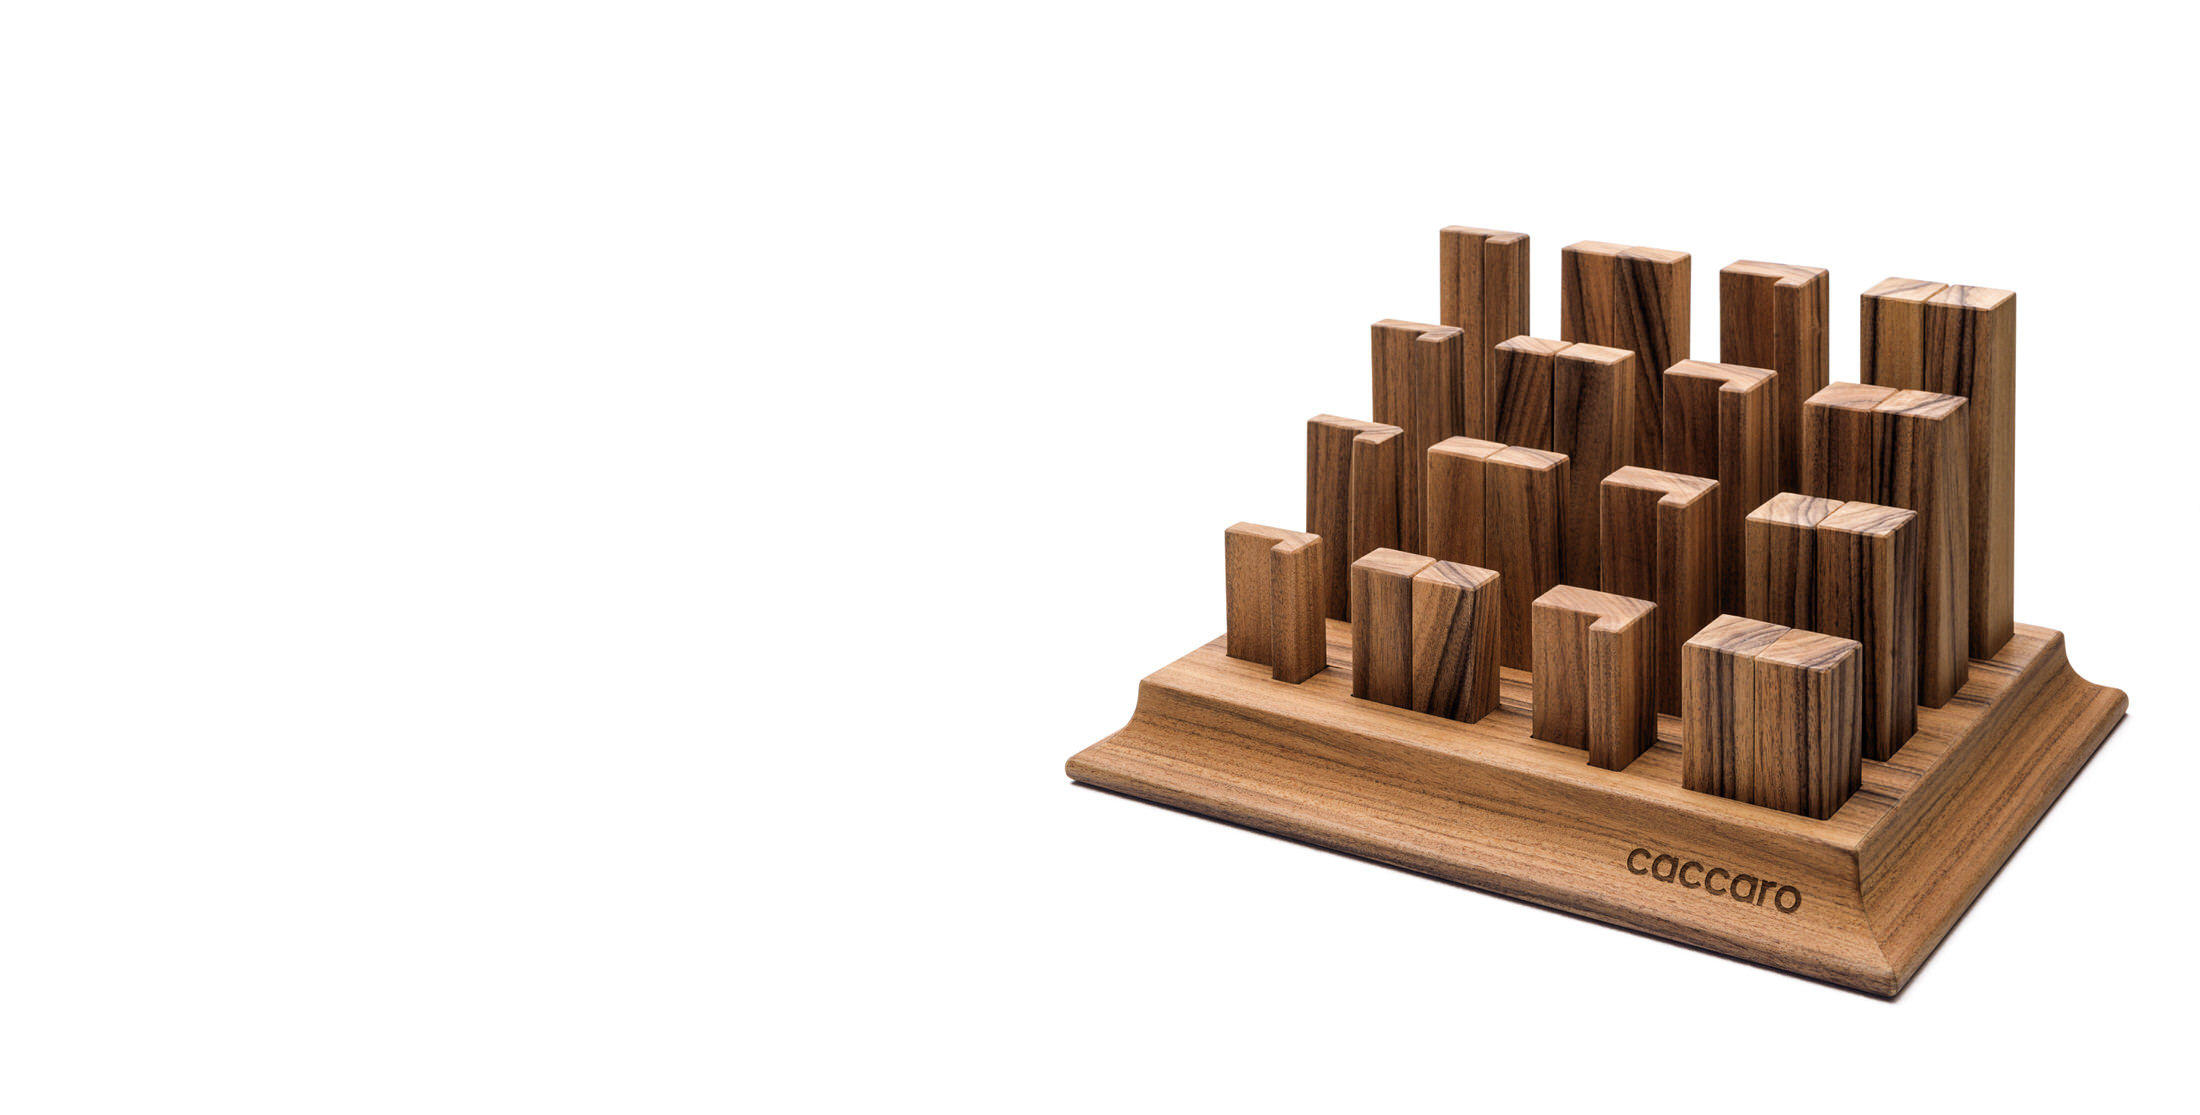
\includegraphics[width=\textwidth]{sez/HomePage/img/Blocchetti.jpg}
	\caption[https://www.caccaro.com/]{Immagine nel first cut: dovrebbe rappresentare la modularità del sistema FreedHome, ma il significato è tutto fuorché immediato.}
	\label{fig:Blocchetti}
\end{figure}

\paragraph*{Altro} Stona particolarmente il paragrafo sotto il first cut (\autoref{fig:Useless}). Veramente troppo largo per essere letto in modo agevole. Oltretutto il contenuto è sostanzialmente inutile.\\
I link che accompagnano i paragrafi hanno la stessa formattazione del testo. Non è inoltre possibile stabilire se una certa pagina è stato visitata o meno.

\begin{figure}[H]
	\centering
	
\includegraphics[width=\textwidth]{sez/HomePage/img/Useless.png}
	\caption[https://www.caccaro.com/]{Liberi di saltare questo paragrafo.}
	\label{fig:Useless}
\end{figure}

